\documentclass{article}
\usepackage[allcolors=true]{hyperref}
\usepackage{graphicx}
\usepackage{amsmath,amsfonts,amsthm,amssymb}
\usepackage{caption}
\usepackage{multirow}
\usepackage{physics}
\usepackage{tikz}
\usepackage{cleveref}
\usepackage{pgfplotstable}
\usepackage{siunitx}
\usepackage{wrapfig}
\usepackage{graphicx}
\usepackage{subfiles}
\usepackage{bm}
\usepackage{xcolor}
\usepackage[french]{babel}
\usepackage{titlesec}
\usepackage{lmodern}
\usepackage{braket}
\usepackage{chngcntr}
\usepackage{geometry}
\geometry{
     a4paper,
    total={170mm,257mm},
    left=20mm,
    top=20mm,
 }

\numberwithin{equation}{part}
\counterwithin*{section}{part}

\pgfplotsset{width=10cm,compat=1.16}

\newcommand{\ti}{\times}
\newcommand{\h}{\hbar}
\renewcommand{\d}{\mathrm{d}}
\renewcommand{\thepart}{\arabic{part}}


\titleformat{\paragraph}
{\normalfont\normalsize\bfseries}{\theparagraph}{1em}{}
\titlespacing*{\paragraph}
{0pt}{3.25ex plus 1ex minus .2ex}{1.5ex plus .2ex}

\title{\textbf{PHYS-F203 - Introduction à la Mécanique Quantique} \\ \textit{Basé sur les notes de Prof. $\href{mailto:serge.massar@ulb.be}{\text{Massar Serge}}$}}
\author{$\href{mailto:juian.moeil@ulb.be}{\text{Moeil Juian}}$ \and $\href{mailto:sami.abdul.sater@ulb.be}{\text{Abdul Sater Sami}}$ \and $\href{mailto:anais.defossez@ulb.be}{\text{Defossez Anais }}$}
\date{\textbf{Année académique 2020-2021}}

\newtheorem{theorem}{Théorème}[section]
\newtheorem{definition}[theorem]{Définition}
\newtheorem{lemma}[theorem]{Lemme}
\newtheorem{Property}[theorem]{Proposition}
\newtheorem{corollary}[theorem]{Corollaire}
\newtheorem{remark}[theorem]{Remarque}
\newtheorem*{preuve}{Preuve}
\newtheorem{reminder}[theorem]{Rappel théorique}
\newtheorem{exemple}[theorem]{Exemple}

\renewcommand\qedsymbol{$\blacksquare$}

\setcounter{tocdepth}{2}

\begin{document}

\maketitle
\begin{center}
    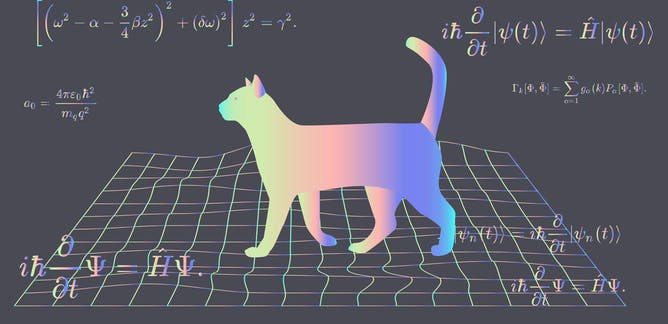
\includegraphics[scale=0.65]{Images/cat.jpg}
\end{center}
\begin{center}
    
\includegraphics[scale=0.2]{Images/sciences.png}
\end{center}
\begin{center}
    
\includegraphics[scale=0.50]{Images/ULB.jpg}
\end{center}

\newpage
\tableofcontents

\newpage
\begin{abstract}
\textit{Ces notes traitent de l'interprétation de Copenhague de la Mécanique Quantique, telle qu'enseignée dans le cadre du cours $\href{https://www.ulb.be/fr/programme/phys-f203}{\text{PHYS-F203}}$ en 2020-2021.} \end{abstract}
\begin{remark}
    Le symbole $\doteq$ est employé pour dire "par définition". Les vecteurs $\bm{x}$ sont indiqués en gras.
\end{remark}

\begin{remark}
    Ces notes ont été rédigées par des étudiant.e.s. Aussi, n'hésitez pas à contacter $\href{mailto:juian.moeil@ulb.be}{\text{MOEIL Juian}}$ pour toute question ou remarque. 
\end{remark}

\textit{Merci à Bellet Björn pour sa relecture.}

\subfile{Chapitre 1/chapitre1.tex}
\newpage
\subfile{Chapitre 2/chapitre2.tex}
\newpage
\subfile{Chapitre 3/chapitre3.tex}
\newpage
\subfile{Chapitre 4/chapitre4.tex}
\newpage
\subfile{Chapitre 5/chapitre5.tex}
\newpage
\subfile{Chapitre 6/chapitre6.tex}
\newpage
\subfile{Chapitre 7/Chapitre7.tex}

\newpage
\subfile{Annexe/annexe.tex}

\end{document}